\documentclass[superscriptaddress,onecolumn,floatfix]{revtex4-2}

\usepackage{graphicx}
\usepackage{epsfig}
\usepackage{color}
\usepackage{amssymb}
\usepackage{amsmath}
\usepackage{array}
\usepackage[loose]{units}
\usepackage{hyperref}
\usepackage{cleveref}
\usepackage{braket}
\usepackage[caption=false]{subfig}
\usepackage[english]{babel}
\usepackage{letltxmacro}

\LetLtxMacro{\ORIGselectlanguage}{\selectlanguage}
\makeatletter
\DeclareRobustCommand{\selectlanguage}[1]{%
    \@ifundefined{alias@\string#1}
      {\ORIGselectlanguage{#1}}
      {\begingroup\edef\x{\endgroup
         \noexpand\ORIGselectlanguage{\@nameuse{alias@#1}}}\x}%
}
\newcommand{\definelanguagealias}[2]{%
  \@namedef{alias@#1}{#2}%
}
\makeatother

\definelanguagealias{en}{english}


\begin{document}
                            
\begin{abstract}
  This manual covers basic use and frequently asked questions for the manual preconditioning kit.
\end{abstract}
\title{Preconditioning Kit Manual}
\author{Electroniq Buttons Boutique}
\email{support@electroniqbuttons.com}
\date{\today}

\maketitle

\section{What is preconditioning?}
In order to protect the battery, an EV's battery management system (BMS) limits DC charging power when the battery is colder or hotter than the optimal temperature for charging (75-95°F). In winter in colder climates, this can mean that charging is far slower than optimal. First-generation E-GMP cars (2021-2024 Ioniq 5/EV6, 2023-2025 Ioniq 6/GV60) can routinely do 10-80\% in 18 minutes under optimal conditions. At worst, you might only see 25kW charging, about ten times slower than the fastest charging speed.

To fix that, Hyundai and Kia added battery heaters to many EVs. Activation of this battery heater in advance of DC charging is called battery preconditioning. Battery preconditioning causes the battery heating system to activate when a charging station is entered into the built-in navigation so that the car arrives at the charger with a warm battery capable of much faster charging than without preconditioning. 

For first-generation E-GMP cars, this feature is only activatable through the built-in navigation. This means that if you navigate to a charger using Google or Apple Maps, or A Better Route Planner, your battery may not be warm enough to reach maximum charging speed. In addition, with many new chargers being built worldwide, the database accessed by the built-in navigation is frequently out of date. In many cases, navigating to a charger with the built-in navigation still will not properly activate your battery heater. This is why we've built a manual button to activate this feature. 

\section{Which cars can use this?} \label{sect:eligibility}
The kit is designed to work on most 2021-2024 Ioniq 5s, 2022-2025 Ioniq 6s, and 2022-2024 EV6s. We have tested on Ioniq 5s from three different markets, as well as one Ioniq 6 and one EV6. \href{mailto:requests@electroniqbuttons.com}{Contact us} if you're interested in using the kit on a different car. The kit will only work if you have a battery heater. To assess that, please check for the `Battery Conditioning Mode' menu in `EV $\to$ EV Settings' (see Fig. \ref{subfig:menus:EVsettings}) on your car's head unit (center screen) (see Fig. \ref{subfig:menus:batt_cond}).
\begin{figure}[h]
  \subfloat[]{\label{subfig:menus:EVsettings}
  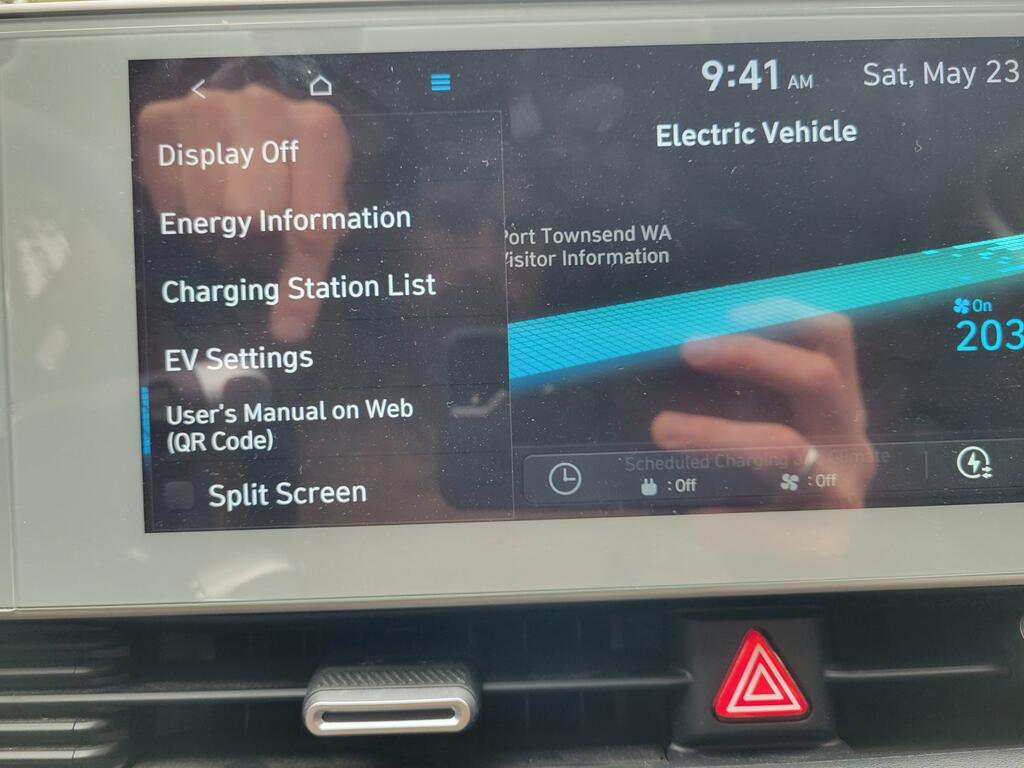
\includegraphics[height=1.95in]{photos/EV_settings.jpg} }
  \subfloat[]{\label{subfig:menus:batt_cond}
  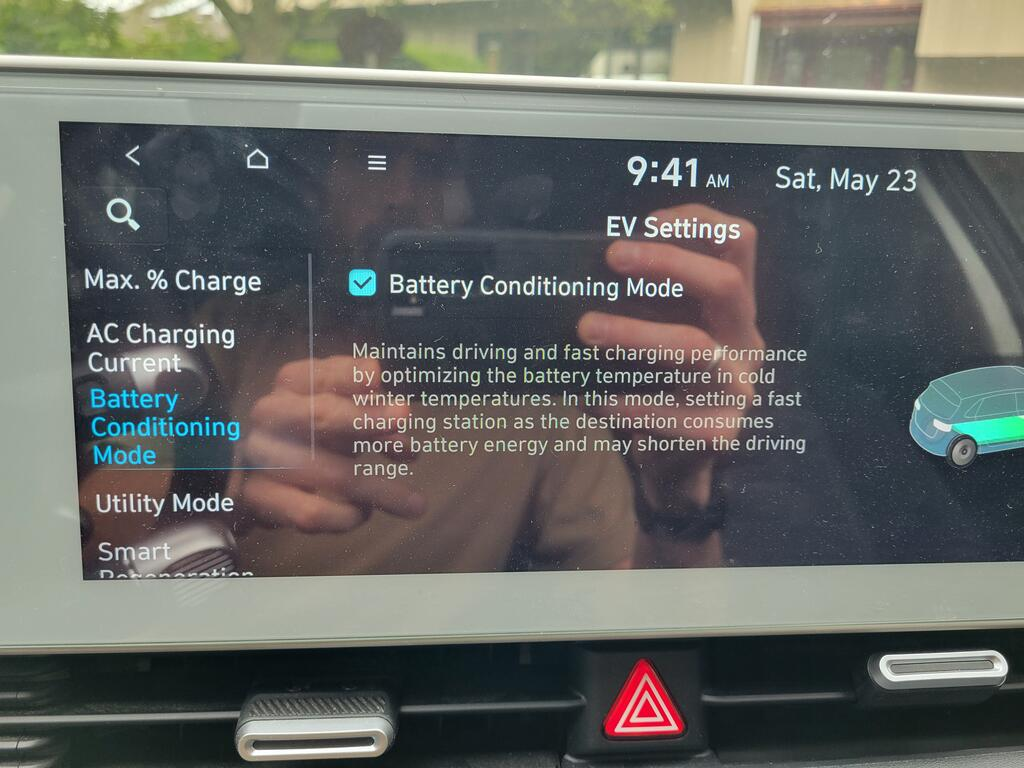
\includegraphics[height=1.95in]{photos/battery_conditioning_mode.jpg} }
   \caption{(a) How to find the EV settings menu: on the main screen, hit the 'EV' icon; then, in the left-hand menu that appears, hit `EV Settings'. (b) `Battery Conditioning Mode' screen. \label{fig:menus}}
\end{figure}

If you do not have this screen, you should not buy this kit. Please contact a dealership or knowledgeable owners in your country to evaluate whether it is possible to install this feature on your car with additional steps. For US, Canada or Norway, feel free to contact us at \href{mailto:support@electroniqbuttons.com}{support@electroniqbuttons.com} and we'll be happy to help you evaluate this with a bit of information about your car.

If instead of `Battery Conditioning Mode' as shown in Figure \ref{subfig:menus:batt_cond}, you have `Winter Mode', your car just needs a firmware update from a dealership. Find the relevant technical service bulletin for your country regarding this update and head to your nearest competent dealership. After completion of this step and confirmation of the `Battery Conditioning Mode' menu replacing `Winter Mode', you can buy this kit.

\section{Basic Kit Setup}
Start with the \href{https://github.com/tylerharvey/Ioniq5_CAN/blob/main/guides/}{installation guides}.  See \href{https://meatpihq.github.io/wican-fw/config/wifi}{WiCAN docs} for basic WiCAN setup. This is not necessary to activate preconditioning, but it's highly recommended that you at least change the default WiFi password for security.  

\section{User Interface}
To activate preconditioning manually, just press the star button on your steering wheel. You should immediately see a countdown in meters/yards on your cluster that hijacks the distance-to-destination indicator. Preconditioning starts when this countdown reaches zero. If the countdown resets, that means something unexpected happened and it's retrying. 

When preconditioning activates, you'll see the standard popup saying, `Battery preconditioning activated for optimal DC charging', shown in Figure \ref{subfig:precon:popup}. You'll also get a snowflake or red coil icon over the battery symbol in the lower lefthand corner of the cluster, shown in Figure \ref{subfig:precon:coil}.

\begin{figure}[h]
  \subfloat[]{\label{subfig:precon:popup}
  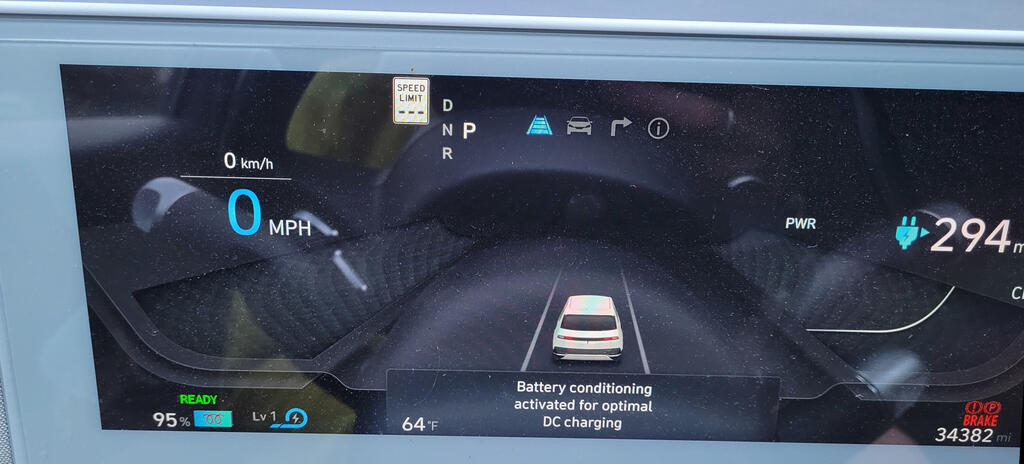
\includegraphics[height=1.95in]{photos/precon_active.jpg} }  \\
  \subfloat[]{\label{subfig:precon:coil}
  
\includegraphics[height=1in]{photos/coil_on_battery.jpg} }
   \caption{(a) Screenshot of the pop-up indicating successful activation of battery preconditioning. (b) Example screenshot of the coil icon overlaid on the battery symbol in the lower left corner of the instrument cluster. \label{fig:precon}}
\end{figure}

If preconditioning never activates, confirm that built-in conditions for activation are met:
\begin{enumerate}
  \item Battery temperature must be less than $\unit[21]{C}$/$\unit[70]{F}$
  \item State of charge must be higher than $\unit[20]{\%}$
  \item `Battery Conditioning Mode' screen is present in `EV Settings' menu (see section \ref{sect:eligibility}
\end{enumerate}
Unfortunately, these are limits that are built into battery management unit firmware or the hardware of the car that we cannot change with this kit.
\section{Frequently Asked Questions}
\begin{enumerate}
  \item[Q:] How do I install it?
  \item[A:] See the \href{https://github.com/tylerharvey/Ioniq5_CAN/blob/main/guides/}{installation guides}. If this looks too complicated, ask your nearest teenager or car audio shop for help!
  \item[Q:] Why does my backup camera, car app, or other center screen feature not work after installation?
  \item[A:] Check the \href{https://github.com/tylerharvey/Ioniq5_CAN/blob/main/guides/harnesses/head_unit_MITM/MITM_harness_modes.pdf}{harness modes guide}. If you have a WiCAN original or no device plugged into the OBD port, the harness must be in parallel mode. If you have a customized WiCAN, the harness should be in MITM mode.
  \item[Q:] Does this make my car easier to steal?
  \item[A:] Not likely, but the installation is designed to be difficult to see for multiple reasons, including security. We highly recommend changing your WiCAN password. 
  \item[Q:] Will this void my warranty?
  \item[A:] Check your country's warranty and consumer protection law. In the US, the Magnusson-Moss Warranty Act offers strong consumer protections. Automaker threats about aftermarket parts "voiding warranties" in many cases do not hold up in court. (This is not legal advice.) At the same time, diagnosis of problems by an automotive technician is challenging, and we highly recommend removal of aftermarket parts and accessories that could make diagnosis more complicated. For example, if you are encountering head unit or USB port problems, it is a good idea to de-install this kit before taking your car into a dealership to avoid complications with diagnosis. 
  \item[Q:] What if I want to build this myself?
  \item[A:] Do it! Everything we've done is \href{https://github.com/tylerharvey/Ioniq5_CAN}{open-source}. Feel free to use the wiring harness diagram to build something yourself. The connectors are available on AliExpress. However, if you make a contribution to public knowledge in the form of a pull request to the \href{https://github.com/dragz/egmpdbc}{DBC file} or something else, rebates are available that will bring the net cost down to competitive-with-DIY pricing with a lot less labor.
  \item[Q:] Why can't this be a software update?
  \item[A:] It could be. We have our guesses as to why Hyundai/Kia hasn't included this in a navigation update. If you  know how to \href{https://discord.gg/zyrngQ5qQ}{hack your head unit} and have found the CAN interface functions, you are welcome to add a manual preconditioning button to your head unit. However, distribution of hacked firmware is not possible at this time, so an aftermarket "update" would be difficult to make widely available.
  \item[Q:] Will this kill my ICCU?
  \item[A:] No.
  \item[Q:] Will this kill my 12V battery?
  \item[A:] Like an OBD reader plugged into the normal OBD port, the WiCAN adds some power usage when the car is off. However, the WiCAN comes with a power saving mode for this purpose. If you're very concerned about this, we encourage you to set the \href{https://meatpihq.github.io/wican-fw/config/sleep-mode}{sleep voltage cutoff} higher to be safer. 
  \item[Q:] Can I use the built-in navigation while using this kit?
  \item[A:] With the beta version, this is not possible. This will be fixed with the customized WiCAN.
  \item[Q:] Will a navigation update affect my ability to use the kit?
  \item[A:] It's highly unlikely, as the kit doesn't depend on communication with the head unit. A battery management unit update could (for instance, the update that enabled preconditioning retroactively on early Ioniq 5s), but we believe those must be done by dealerships. However, we can't promise with 100\% certainty that a navigation update will not affect the functionality of the kit. In the off chance that this does happen, let us know and we will do our best to update logic to restore manual preconditioning functionality.
  \item[Q:] Will you build me a new button?
  \item[A:] Maybe! Email us at \href{mailto:requests@electroniqbuttons.com}{requests@electronicbuttons.com} with your requests.
  \item[Q:] Your business is called `Electroniq Buttons Boutique'. Where are the physical buttons?
  \item[A:] We are working on making physical buttons available. Roy has a tested prototype shown in his \href{https://github.com/dragz/ironiq}{Ironiq} repository.
\end{enumerate}
% \begin{figure}[h]
%   \subfloat[]{\label{subfig:overview:harness}
%   \includegraphics[height=1.95in]{photos/whole_harness.jpg} }
%   \subfloat[]{\label{subfig:overview:shunt_cap_labeled}
%   \includegraphics[height=1.95in]{photos/labeled_connectors_MITM_harness.jpg} }
%    \caption{(a) Man-in-the-middle harness. (b) Overview of connectors showing shunt cap. \label{fig:overview}}
% \end{figure}
\appendix 
\bibliographystyle{apsrev4-1}
\bibliography{stemh_model}{}
\end{document}
